\documentclass{article}
\usepackage[french]{babel}
\usepackage[utf8]{inputenc}
\usepackage{times}
\usepackage{geometry}
\usepackage{lmodern}
\usepackage[T1]{fontenc}
\usepackage{graphicx} % Package pour insérer des images

\geometry{a4paper, margin=2.5cm}

\title{
    Rapport de TIR
}
\author{DIALLO Abdoul Aziz \and JERE Corentin \and BRIGTHON Cannelle \and LECOMTE Alex \and DOMINGUEZ Vincent}
\date{\today}
\begin{document}

\maketitle

\begin{center}
    \vspace*{\fill} % Espace vertical avant l'image
    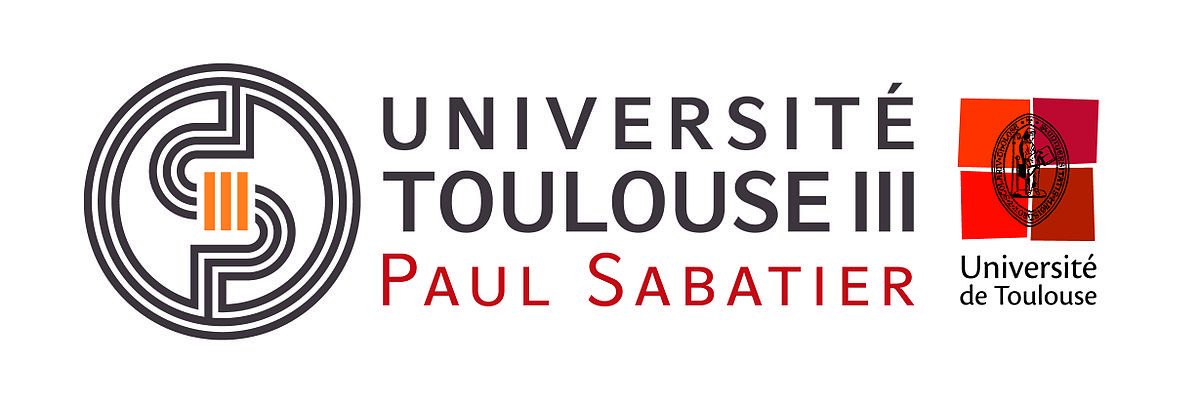
\includegraphics[width=0.6\textwidth]{Logo_UT3.jpg}
    \vspace*{\fill} % Espace vertical après l'image
\end{center}

\newpage
\tableofcontents
\newpage

\section{Présentation globale des problématiques abordées}

Les articles de recherche présentés abordent principalement les problématiques liées à la manipulation et à l'édition de l'apparence des matériaux et de l'éclairage dans les environnements virtuels. Cette thématique se situe à l'intersection de l'informatique graphique, de la perception visuelle et de l'apprentissage automatique. 

L'apparence des matériaux et l'éclairage jouent un rôle fondamental dans notre perception et notre compréhension du monde qui nous entoure. Cependant, la manipulation intuitive de cette apparence reste un défi majeur en informatique graphique, notamment en raison de la complexité des interactions entre la lumière et la matière.

Les recherches examinées se concentrent sur plusieurs aspects clés. Premièrement, elles abordent la difficulté de comprendre et de modéliser mathématiquement les attributs perceptuels de haut niveau qui définissent l'apparence visuelle des matériaux, comme l'aspect "métallique", "brillant" ou "rugueux". Ces attributs sont souvent ambigus et subjectifs, ce qui complique leur représentation algorithmique. Deuxièmement, les articles explorent les défis associés à la manipulation des propriétés des matériaux à partir d'une seule image ou photo prise "dans la nature", sans contrôle sur les conditions d'éclairage ou la géométrie. Troisièmement, les travaux tentent de résoudre le problème du "rendu inverse", qui consiste à estimer ou modifier les paramètres physiques des matériaux à partir d'images, en tenant compte des facteurs confondants comme l'éclairage et la géométrie de la scène.

Ces recherches tentent également de résoudre un problème fondamental en infographie : comment permettre aux artistes et designers de contrôler efficacement l'apparence visuelle d'une scène rendue par ordinateur, en particulier en ce qui concerne les effets lumineux complexes. Bien que les algorithmes de rendu physiquement réalistes aient considérablement progressé pour simuler l'illumination globale, ces méthodes ne fournissent pas suffisamment de contrôle artistique. En effet, la simulation physiquement correcte de la propagation de la lumière (transport lumineux) génère des résultats réalistes mais difficilement modifiables selon les intentions artistiques. Les artistes se retrouvent souvent contraints d'ajuster laborieusement des paramètres bas niveau (positions des sources lumineuses, propriétés des matériaux) par un processus fastidieux d'essai-erreur pour obtenir l'effet visuel souhaité.

Les recherches présentées abordent cette problématique en proposant différentes approches pour éditer et manipuler les effets d'éclairage et l'apparence des matériaux de manière plus intuitive. Elles couvrent plusieurs aspects comme :
\begin{itemize}
\item L'édition et la manipulation directe des ombres et des reflets
\item Le contrôle de l'éclairage indirect et des effets de caustique
\item La manipulation du transport lumineux dans l'espace des chemins (\textit{path-space})
\item La redirection des rayons lumineux pour modifier l'apparence sans changer la configuration géométrique
\item L'édition artistique des matériaux et de leur interaction avec la lumière
\end{itemize}

Les recherches s'orientent progressivement vers des approches basées sur le deep learning et les réseaux neuronaux génératifs pour capturer et manipuler les attributs d'apparence des matériaux. Cette tendance reflète la difficulté inhérente à modéliser explicitement les relations complexes entre les paramètres physiques des matériaux et leur perception visuelle par les humains.

Ces travaux ont un objectif commun : développer des méthodes qui permettent un contrôle artistique intuitif tout en préservant la cohérence visuelle des résultats dans un cadre d'illumination globale. Ils cherchent à trouver un équilibre entre le réalisme physique et la liberté créative.

\newpage
\section{Portée de la recherche bibliographique}

La recherche bibliographique couvre un large éventail d'approches et de méthodologies développées pour l'édition et la manipulation de l'apparence des matériaux et de l'éclairage. Les articles sélectionnés s'étendent de 1991 à 2023, permettant ainsi de suivre l'évolution des techniques dans ce domaine en rapide progression.

Sur le plan méthodologique, l'étude englobe différentes approches: des techniques basées sur la physique utilisant des BRDFs (Bidirectional Reflectance Distribution Functions) paramétriques ainsi que non paramétriques aux méthodes de deep learning comme les réseaux adversaires génératifs (GANs) et les réseaux de neurones convolutifs. Les articles abordent également diverses techniques de transfert de style, d'édition basée sur les attributs perceptuels, et de manipulation directe dans l'espace image.

Le corpus documentaire couvre plusieurs niveaux de représentation des matériaux: depuis les modèles analytiques comme Cook-Torrance ou GGX jusqu'aux représentations apprises de manière implicite par des deep learning network. Cette diversité permet d'examiner les forces et les faiblesses de chaque approche selon différents contextes d'application.

Les publications analysées comprennent des travaux fondamentaux comme :

\begin{itemize}
\item \textit{Design and Simulation of Opera Lighting and Projection Effects} (Dorsey et al., 1991) - Un travail précurseur sur la conception et la simulation d'effets d'éclairage pour les productions d'opéra.

\item \textit{Metropolis Light Transport} (Veach et Guibas, 1997) - Un algorithme fondamental pour le transport lumineux basé sur l'échantillonnage de Metropolis, qui constitue une base théorique importante pour le rendu réaliste et l'édition d'éclairage.

\item \textit{State of the Art in Artistic Editing of Appearance, Lighting, and Material} (Schmidt et al., 2014) - Une synthèse complète des méthodes d'édition artistique de l'apparence visuelle, couvrant l'éclairage, les matériaux et leurs interactions.

\item \textit{iCheat: A Representation for Artistic Control of Indirect Cinematic Lighting} (Obert et al., 2008) - Une approche pour le contrôle artistique de l'éclairage indirect dans des applications cinématographiques.

\item \textit{RayPortals: A Light Transport Editing Framework} (Subileau et al., 2017) - Une méthode récente permettant d'éditer le transport lumineux en redirigeant des rayons de lumière dans l'espace 3D.
\end{itemize}

Les recherches incluent également des études sur la perception humaine des matériaux, explorant comment les attributs de haut niveau comme la brillance, l'aspect métallique ou la rugosité sont perçus et interprétés par le système visuel humain. Ces études perceptuelles fournissent une base essentielle pour développer des interfaces d'édition plus intuitives et alignées avec la cognition humaine.

La recherche couvre également un spectre d'applications variées, des productions théâtrales et opéras aux rendus cinématographiques et à la synthèse d'images photoréalistes pour les médias numériques. Cette diversité permet d'explorer comment les méthodes d'édition d'éclairage et de matériaux ont évolué pour répondre aux besoins spécifiques de différents contextes artistiques.

Géographiquement, les travaux proviennent de divers groupes de recherche internationaux, principalement d'Amérique du Nord, d'Europe et d'Asie, offrant ainsi une perspective globale sur l'état de l'art. Les publications sont issues de conférences et journaux prestigieux en informatique graphique comme SIGGRAPH, Eurographics, Computer Graphics Forum et ACM Transactions on Graphics.
\newpage
\section{Material Editing in Complex Scenes by Surface Light Field Manipulation and Reflectance Optimization}

Cet article présente une nouvelle approche pour l'édition intuitive des matériaux dans des scènes 3D complexes. Contrairement aux méthodes traditionnelles qui se concentrent sur la modification directe des propriétés de réflectance (comme la brillance ou la diffusion), le système proposé permet aux utilisateurs de manipuler directement l'apparence visuelle de la scène via des coups de pinceau sur la surface.

Les principales applications incluent la peinture diffuse, la conception de reflets spéculaires, la manipulation de l'éclairage indirect, et la création de caustiques. Le système fonctionne avec des géométries complexes, des matériaux à variation spatiale et des éclairages environnementaux.

Cette approche permet aux artistes de se concentrer sur l'apparence visuelle désirée plutôt que sur les paramètres techniques des matériaux, tout en garantissant que les modifications aboutissent à des matériaux physiquement plausibles.

\section{Path-Space Manipulation of Physically-Based Light Transport}
Ce document présente une méthode innovante pour manipuler le transport de lumière en infographie 3D, particulièrement dans les rendus physiquement réalistes (PBR). Les auteurs proposent des outils permettant aux artistes d'éditer intuitivement des effets d'éclairage complexes comme les caustiques, les réflexions et les ombres, tout en maintenant un aspect physiquement plausible.

Le système fonctionne en opérant directement sur l'espace des chemins de lumière et propose deux approches complémentaires : le ``path retargeting'' qui permet de transformer (déplacer, tourner, redimensionner) directement les chemins de lumière, et le ``path-proxy linking'' qui modifie indirectement le transport lumineux en liant des phénomènes spécifiques à des objets proxy dans la scène. 

L'outil inclut également des fonctionnalités de sélection intelligente et de visualisation des chemins lumineux, permettant aux artistes d'identifier et de comprendre les phénomènes qu'ils souhaitent modifier. Le système s'intègre aux logiciels de création 3D professionnels et supporte les animations et les scènes dynamiques.

Les tests utilisateurs réalisés avec des directeurs techniques spécialisés en éclairage confirment que cette approche améliore significativement le workflow artistique dans les systèmes de rendu physiquement réalistes, permettant des ajustements précis et rapides qui seraient autrement difficiles à obtenir.

\section{RayPortals: a light transport editing framework}
Le papier présente RayPortals, un framework permettant de modifier le transport de la lumière dans les rendus 3D. Contrairement aux approches traditionnelles qui modifient les sources de lumière ou les matériaux pour obtenir des effets visuels spécifiques, RayPortals permet de manipuler directement la propagation des rayons lumineux dans l'espace.

Le concept central repose sur des ``portails'' - des paires de surfaces paramétrées dans l'espace 3D. Un portail capture les rayons lumineux à un endroit (surface d'entrée) et les téléporte vers un autre endroit (surface de sortie), permettant ainsi de déplacer, dupliquer ou modifier des effets d'éclairage comme les caustiques, les réflexions ou les saignements de couleur. Le système inclut également un mécanisme de filtrage basé sur des expressions régulières pour sélectionner précisément les chemins lumineux à modifier.

Les auteurs ont implémenté RayPortals dans trois algorithmes de rendu majeurs : Photon Mapping, Progressive Photon Mapping et Bi-directional Path Tracing. Les résultats démontrent que cette approche unifie et étend les techniques précédentes de manipulation d'éclairage, offrant un contrôle artistique précis sans nécessiter de modifier la géométrie de la scène ou la configuration des lumières. L'impact sur les performances reste raisonnable, avec une surcharge de calcul d'environ 12-20\% selon les techniques de rendu utilisées.

\newpage
\section{Controlling Material Appearance by Examples}
Ce document présente une méthode pour améliorer et contrôler l'apparence de matériaux 3D existants en utilisant des photographies comme références. Les auteurs ont développé une version modifiée de MaterialGAN, un réseau neuronal générateur, qui préserve la capacité de ``tuilage'' (tileability) des textures - caractéristique essentielle pour l'application de matériaux sur de grandes surfaces sans raccords visibles.

La méthode proposée transfère les micro et méso-structures de texture des photos cibles vers les cartes de matériaux existantes (albédo, normale, rugosité et spécularité), tout en conservant la structure globale du matériau d'origine. Pour ce faire, les auteurs optimisent l'espace latent de MaterialGAN en utilisant un rendu différentiable qui compare les statistiques visuelles entre le rendu et les images cibles.

L'approche permet également un contrôle spatial précis, permettant de transférer l'apparence de plusieurs photos cibles vers différentes régions d'un même matériau. Les applications incluent l'amélioration de matériaux procéduraux qui manquent souvent de réalisme, la création de nouveaux matériaux à partir de références photographiques simples, et la conception de scènes 3D avec des matériaux cohérents et réalistes.

\newpage
\section{Analysis of the path space for light and shadow compositing}
Cet article nous présente les principales méthodes et approches permettant de modifier la lumière ainsi que les ombres dans une animation.

Il se concentre sur les avantages que chaque approche a apporté ainsi que les inconvénients qui ont ainsi mener à l’élaboration de nouvelles méthodes encore et encore, faisant de ce domaine un domaine avec des améliorations constantes.

D’ailleurs la première partie après l’introduction est un état de l’Art, nous permettant de nous familiariser avec les notions de ce domaine qu’est l’édition de la lumière.

Ces premières approches sont donc méthode d’Anjyo, la méthode Kawai, l’Inverse rendering, Differentiable Rendering ou encore RayPortals.

L’état de l’Art est alors assez complet et chaque point est clairement détaillé offrant une compréhension net du sujet.

Ce qui ressort de cet état de l’art est que malgré les différentes approches, un problème persiste : le coût en temps de calculs et en mémoire.

Ce qui nous amène à la partie 3. Pour résoudre cet obstacle, des chercheurs ont mis au point le path Space Clustering qui permet d’améliorer le compositing en post-production en organisant mieux les informations de lumière dans une scène 3D.

Ces informations sont stockées sous forme de Arbitrary Output Variables.

La simulation le transport de la lumière et son interaction sur les surfaces, différentes équations physiques comme la radiance et la formule du rendu.

De plus, pour réduire le nombre de chemins lumineux, des expressions régulières sont utilisés. Cette approche a donc été testé sur sur 2 scènes : Coffee Maker et Marbles via le moteur pbrt-v3.

Les résultats sont très concluants, néanmoins il y a toujours un inconvénient qui est que les ombres ne peuvent pas être capter directement.

La partie 4 présente alors à nouveau une nouvelle méthode pour répondre à ce problème : les shadow layers.

A l’origine pour représenter des ombres, on utilisait des couches de niveau de gris mais cela manquant de réalisme, les shadow layers se sont imposés.

On a ainsi approche beaucoup plus physique des ombres car les shadow layers représentent la perte d’énergie lumineuse dû à un objet.

La Scène est alors divisée en plusieurs types d’objets : la source lumineuse, le shadow caster (bloque la lumière), le shadow catcher (reçoit la lumière), l’auto-ombre (l’ombre d’un objet sur lui-même) et l’ombre portée (l’ombre d’un objet sur un autre).

Pour calculer un shadow layer, on vient comparer la version de la scène sans l’objet puis la version où l’objet est un trou noir. Les résultats sont bien présentés et sont concluants.

Pour compléter cette approche, la partie 5 étend les shadow layers aux médias participatifs (le gaz, la fumée…) en utilisant une approche par intégrale de chemins. La dernière partie explique les axes d’amélioration comme améliorer la description des LPE, utiliser la covariance de la lumière ou ajouter un outil de pré-filtrage.

Pour conclure, cet article est compréhensible, bien détaillé avec des figures clairs et cite ses références.

Certains résultats sont cependant rapidement expliqués et ne font pas forcément l’objet d’une conclusion.

\newpage
\section{In-the-wild Material Appearance Editing using Perceptual Attributes}
Cet article traite de la modification de l’apparence des matériaux d’objets dans une animation.

Pour commencer, on nous expose l’état de l’art ainsi que les problèmes qui en découlent.

Habituellement, c’est de la géométrie qui est utilisée pour modifier l’apparence des matériaux mais cela apporte son lot d’erreur.

Ainsi l’approche que nous expose cet article est d’utiliser un modèle de réseau neuronal génératifs et une architecture utilisant des cellules "Selective Transfer Unit" (STU).

Ce modèle sera entrainé grâce à une base de donnée de photo du monde réel. Cette base de donnée est composée de 45 500 images générées avec 13 géométries et 7 éclairages.

Les images sont annotées par 2600 humains qui leur mettent une note de perception.

De plus, une relation encodeur-decodeur est utilisée pour déconstruire l’image sous forme de code puis la reconstruire avec le nouvel aspect du matériau passé en paramètre. Le modèle est ainsi entrainé durant 2 jours. Cet entrainement est réalisé avec PyTorch, une RTX 3090 et est optimisé avec ADAM.

Pour ce qui est des résultats, les images synthétisées ont été comparées avec des images provenant de Mitsuba 3 et cela correspond globalement, offrant alors un meilleur résultat que les approches précédentes.

De plus, les cellules STU ont prouvés leur efficacité car sans elles le décodage est moins précis.

L’article présente malgré tout les inconvénients qu’il reste à améliorer, notamment, que la modification s’avère difficile si la surface est trop brillante.

Aussi, les attributs passés en paramètre avaient parfois un sens trop proche comme par exemple : le brillant et le métal rendant encore une fois compliqué la modification.

A noter également que l’article présente la base de donnée comme étant trop homogène et refaire les tests avec un des datasets plus variés est donc une bonne piste d’amélioration.

Enfin l’article nous précise que pour raison technique, la résolution des images était limitée.

Pour conclure, bien qu’appropriée, la méthodologie manque un peu de clarté tout comme les résultats qui ne sont pas très clairement décrits rendant la compréhension plus difficile. L’état de l’art est aussi peu développée. Cependant, les limites de l’approche sont très claires et complètes.

\newpage
\section{State of the Art in Artistic Editing of Appearance, Lighting, and Material}
Ce document est un état de l'art qui présente une vue complete des techniques d'édition artistique de l'apparence, de l'éclairage et des matériaux dans le domaine
de l'informatique graphique.

Premièrement, le rapport s'interesse aux méthodes permettant de modifier l'apparence finale d'une image ou d'une séquence d'animation.
L'objectif de l'édition d'apparence est d'ajuster les matériau et l'éclairage dans le but d'obtenir un resultat répondant à des critères artistiques
précis, que ce soit pour le cinéma (auquel il y a un article dedié), l'architecture ou d'autres industries créatives.

Ensuite, le document présente divers systèmes qui permettent de manipuler les éclairages, allant des approches simples comme le “light linking” aux 
méthodes plus complexes intégrant la simulation globale de l’illumination (global illumination). Ces techniques intègrent des interfaces 
de type « click-and-drag », de la manipulation directe ou indirecte, et même des méthodes basées sur le dessin (painting) pour adapter les ombres 
et les reflets.

La modification des matériaux s’avère particulièrement complexe du fait de la nature non linéaire des interactions entre lumière et surface. 
Le rapport aborde : L’édition directe des paramètres (par exemple, ajuster les composantes d’un BRDF), des méthodes indirectes et basées sur des 
contraintes, qui permettent à l’utilisateur de définir des zones ou des effets visuels souhaités avant que le système ne détermine les paramètres
adéquats et des techniques "data-driven" qui exploitent des bases de données ou des modèles prédéfinis pour faciliter l’édition.

Le rapport identifie également plusieurs défis clés, notamment la complexité du transport de la lumière, la non-linéarité des interactions 
matériaux-lumière et le besoin impératif d’un rendu interactif de qualité. Il propose ainsi une synthèse des travaux existants et met en lumière
les problématiques ouvertes qui guideront les recherches futures pour obtenir des outils d’édition d’apparence plus intuitifs et performants.

\newpage
\section{Conclusion sur l'état de l'art}

L'analyse chronologique des articles révèle une évolution significative des approches pour la manipulation de l'apparence des matériaux et de l'éclairage en informatique graphique.

En 1991, Dorsey et al. posaient les bases conceptuelles avec des techniques de simulation d'éclairage théâtral, marquant les premiers pas vers des outils dédiés aux artistes dans un contexte de rendu informatique. Ces travaux pionniers étaient limités par les capacités matérielles de l'époque et se concentraient principalement sur l'éclairage direct.

L'algorithme de Metropolis Light Transport (Veach et Guibas, 1997) a ensuite constitué une avancée théorique majeure, permettant un échantillonnage plus efficace des chemins lumineux complexes, bien que l'accent soit davantage mis sur la simulation physique que sur le contrôle artistique.

Avec iCheat (Obert et al., 2008), un changement de paradigme s'observe, où le contrôle artistique devient l'objectif principal. Cette approche a introduit une représentation permettant aux artistes de manipuler l'éclairage indirect cinématographique, comblant ainsi l'écart entre la simulation physique et l'intention artistique.

La synthèse de Schmidt et al. (2014) démontre la maturité atteinte par le domaine, cataloguant une vaste gamme de techniques développées au cours des deux décennies précédentes. Ce travail de fond met en évidence la complexité des défis restants et les directions futures de recherche.

Entre 2016 et 2017, avec des travaux comme RayPortals (Subileau et al., 2017) et ceux de Lagunas et al. et Hu et al., la recherche était encore largement axée sur des modèles paramétriques physiquement réalistes et des techniques de décomposition de la lumière. Ces approches nécessitaient souvent une estimation explicite de la géométrie et de l'illumination de la scène, limitant leur applicabilité aux environnements contrôlés.

Entre 2018 et 2020, on observe une transition notable vers les méthodes basées sur le deep learning. Des travaux comme ceux de Delanoy et al. (2020) et Deschaintre et al. (2020) ont commencé à exploiter les réseaux adversaires génératifs et les réseaux neuronaux convolutifs pour capturer et manipuler l'apparence des matériaux directement à partir d'images, sans nécessiter une estimation explicite des paramètres physiques. Cette période marque un changement de paradigme important, passant des modèles physiques explicites aux représentations implicites apprises.

Les travaux les plus récents, comme ceux de Subias et Lagunas (2023) et Hu et al. (2022), représentent l'état de l'art actuel. Ces recherches utilisent des architectures neuronales avancées, comme les cellules de transfert sélectif (STU) et les réseaux génératifs spécialisés, pour permettre l'édition intuitive des attributs perceptuels de haut niveau directement dans l'espace image, sans nécessiter une connaissance approfondie des modèles de réflectance sous-jacents. Ces méthodes récentes sont capables de fonctionner avec des photographies "dans la nature" et des vidéos, où les conditions d'éclairage et la géométrie ne sont pas contrôlées.

Un aspect particulièrement prometteur des travaux récents est l'intégration des connaissances sur la perception humaine des matériaux dans les systèmes d'édition. Des approches comme celle de Hu et al. dans "Controlling Material Appearance by Examples" (2022) utilisent des données collectées auprès d'utilisateurs humains pour entraîner des modèles qui alignent les manipulations des attributs perceptuels avec nos attentes visuelles.

On observe ainsi une tendance claire dans l'évolution des techniques : d'une approche initialement orientée simulation physique vers des méthodes hybrides qui préservent le réalisme tout en offrant un contrôle artistique accru. Cette progression reflète plus largement l'évolution de l'informatique graphique, qui passe progressivement de la recherche de l'exactitude physique à la création d'outils expressifs permettant aux artistes de manipuler efficacement l'apparence visuelle des scènes rendues, tout en conservant la richesse visuelle qu'offre l'illumination globale.

En conclusion, bien que des progrès significatifs aient été réalisés, le domaine de l'édition de l'apparence des matériaux et de l'éclairage reste confronté à des défis importants, notamment la généralisation à des scènes complexes, la manipulation précise des propriétés optiques complexes comme la translucidité, l'édition de matériaux anisotropes, la performance en temps réel, la simplicité d'utilisation pour les artistes non techniques, et l'intégration de ces méthodes dans les pipelines de production existants. Les recherches futures pourraient bénéficier d'une intégration plus poussée des modèles de perception humaine et des avancées en apprentissage génératif pour créer des outils d'édition encore plus intuitifs et puissants.

\end{document}